\documentclass[tikz,border=10pt]{standalone}
\usepackage[utf8]{inputenc}
\usepackage[T1]{fontenc}
\usepackage{lmodern}
\usepackage{tikz}
\usetikzlibrary{shapes.geometric, arrows.meta, positioning, calc, fit, backgrounds}

\begin{document}
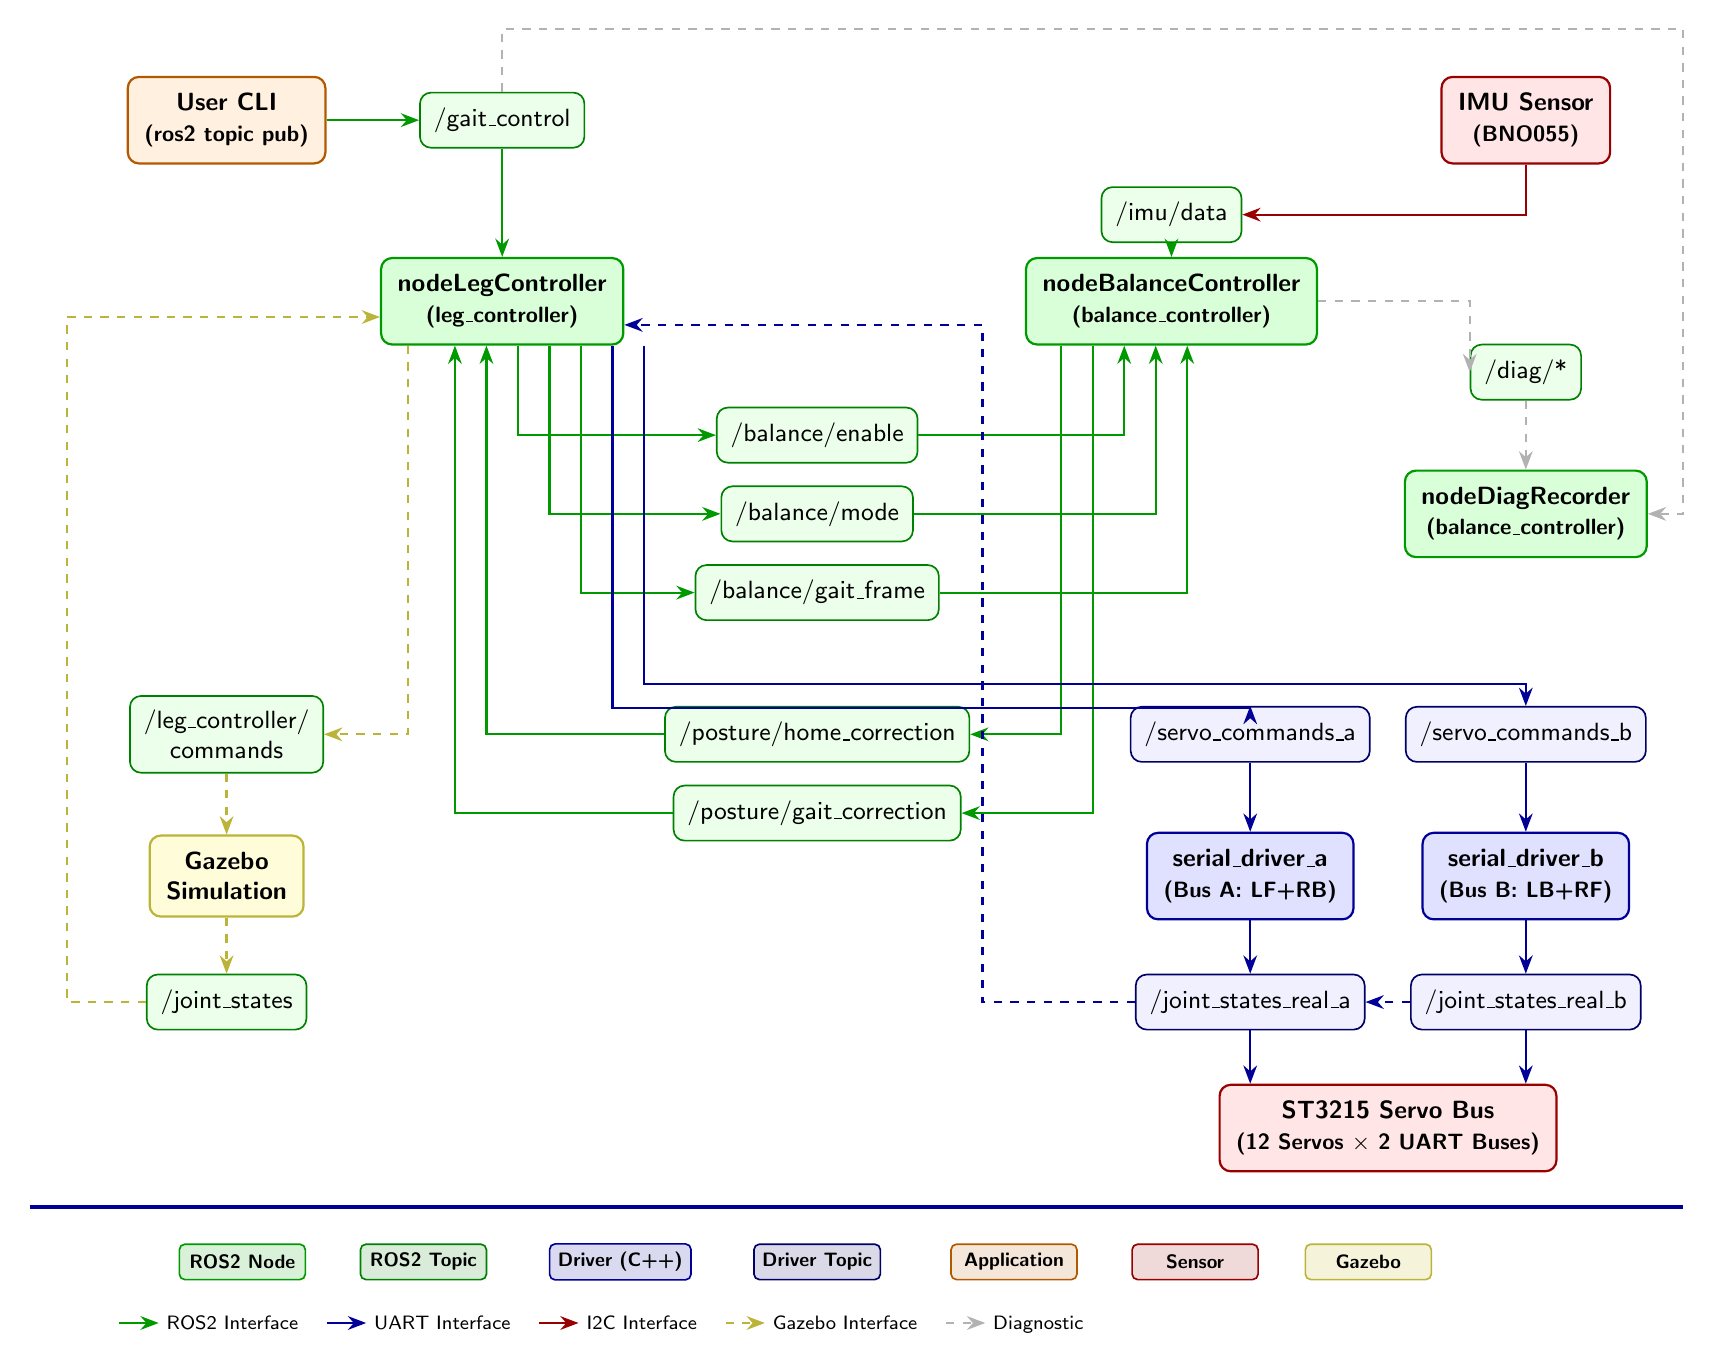
\begin{tikzpicture}[
    font=\sffamily\small,
    >=Stealth,
    % ── Node styles ──
    ros2node/.style={rectangle, rounded corners=4pt, draw=green!60!black, fill=green!15, 
        inner sep=6pt, minimum height=0.9cm, align=center, font=\sffamily\small\bfseries,
        line width=0.8pt},
    ros2topic/.style={rectangle, rounded corners=4pt, draw=green!50!black, fill=green!8, 
        inner sep=5pt, minimum height=0.7cm, align=center, font=\sffamily\small,
        line width=0.6pt},
    cppnode/.style={rectangle, rounded corners=4pt, draw=blue!60!black, fill=blue!12, 
        inner sep=6pt, minimum height=0.9cm, align=center, font=\sffamily\small\bfseries,
        line width=0.8pt},
    cpptopic/.style={rectangle, rounded corners=4pt, draw=blue!40!black, fill=blue!6, 
        inner sep=5pt, minimum height=0.7cm, align=center, font=\sffamily\small,
        line width=0.6pt},
    appbox/.style={rectangle, rounded corners=4pt, draw=orange!70!black, fill=orange!12, 
        inner sep=6pt, minimum height=0.9cm, align=center, font=\sffamily\small\bfseries,
        line width=0.8pt},
    sensorbox/.style={rectangle, rounded corners=4pt, draw=red!60!black, fill=red!10, 
        inner sep=6pt, minimum height=0.9cm, align=center, font=\sffamily\small\bfseries,
        line width=0.8pt},
    gazebobox/.style={rectangle, rounded corners=4pt, draw=yellow!70!black, fill=yellow!15, 
        inner sep=6pt, minimum height=0.9cm, align=center, font=\sffamily\small\bfseries,
        line width=0.8pt},
    % ── Arrow styles ──
    rosarr/.style={->, thick, draw=green!60!black},
    cpparr/.style={->, thick, draw=blue!60!black},
    snsarr/.style={->, thick, draw=red!60!black},
    gazarr/.style={->, thick, draw=yellow!70!black, dashed},
    diagarr/.style={->, thick, draw=gray!60, dashed},
    % ── Legend ──
    legbox/.style={rectangle, rounded corners=2pt, draw=#1, fill=#1!15, 
        inner sep=3pt, minimum width=1.6cm, minimum height=0.45cm, align=center, 
        font=\sffamily\scriptsize\bfseries, line width=0.6pt},
]

% ═══════════════════════════════════════════════════════════
%  Row 1: User Input + IMU Sensor
% ═══════════════════════════════════════════════════════════

\node[appbox] (user) at (0, 0) {User CLI\\{\footnotesize(ros2 topic pub)}};
\node[ros2topic] (gait_ctl) at (3.5, 0) {/gait\_control};
\node[sensorbox] (imu_hw) at (16.5, 0) {IMU Sensor\\{\footnotesize(BNO055)}};

% ═══════════════════════════════════════════════════════════
%  Row 2: Main Nodes
% ═══════════════════════════════════════════════════════════

\node[ros2node] (leg_node) at (3.5, -2.3) {nodeLegController\\{\footnotesize(leg\_controller)}};
\node[ros2topic] (imu_topic) at (12.0, -1.2) {/imu/data};
\node[ros2node] (bal_node) at (12.0, -2.3) {nodeBalanceController\\{\footnotesize(balance\_controller)}};

% ═══════════════════════════════════════════════════════════
%  Row 3: Control topics (leg → balance)
% ═══════════════════════════════════════════════════════════

\node[ros2topic] (bal_en) at (7.5, -4.0) {/balance/enable};
\node[ros2topic] (bal_mode) at (7.5, -5.0) {/balance/mode};
\node[ros2topic] (gait_frame) at (7.5, -6.0) {/balance/gait\_frame};

% ═══════════════════════════════════════════════════════════
%  Row 4: Correction topics (balance → leg)
% ═══════════════════════════════════════════════════════════

\node[ros2topic] (home_corr) at (7.5, -7.8) {/posture/home\_correction};
\node[ros2topic] (gait_corr) at (7.5, -8.8) {/posture/gait\_correction};

% ═══════════════════════════════════════════════════════════
%  Simulation path (left column)
% ═══════════════════════════════════════════════════════════

\node[ros2topic] (leg_cmd) at (0, -7.8) {/leg\_controller/\\commands};
\node[gazebobox] (gazebo) at (0, -9.6) {Gazebo\\Simulation};
\node[ros2topic] (jnt_st) at (0, -11.2) {/joint\_states};

% ═══════════════════════════════════════════════════════════
%  Real hardware path (right column)
% ═══════════════════════════════════════════════════════════

\node[cpptopic] (srv_a) at (13.0, -7.8) {/servo\_commands\_a};
\node[cpptopic] (srv_b) at (16.5, -7.8) {/servo\_commands\_b};

\node[cppnode] (drv_a) at (13.0, -9.6) {serial\_driver\_a\\{\footnotesize(Bus A: LF+RB)}};
\node[cppnode] (drv_b) at (16.5, -9.6) {serial\_driver\_b\\{\footnotesize(Bus B: LB+RF)}};

\node[cpptopic] (fb_a) at (13.0, -11.2) {/joint\_states\_real\_a};
\node[cpptopic] (fb_b) at (16.5, -11.2) {/joint\_states\_real\_b};

\node[sensorbox] (servos) at (14.75, -12.8) {ST3215 Servo Bus\\{\footnotesize(12 Servos $\times$ 2 UART Buses)}};

% ═══════════════════════════════════════════════════════════
%  Diagnostic Recorder (far right)
% ═══════════════════════════════════════════════════════════

\node[ros2topic] (diag_t) at (16.5, -3.2) {/diag/*};
\node[ros2node] (diag_rec) at (16.5, -5.0) {nodeDiagRecorder\\{\footnotesize(balance\_controller)}};

% ═══════════════════════════════════════════════════════════
%  Connections — Layer 1
% ═══════════════════════════════════════════════════════════

% User → gait_control → leg_node
\draw[rosarr] (user) -- (gait_ctl);
\draw[rosarr] (gait_ctl) -- (leg_node);

% IMU sensor → /imu/data → balance node
\draw[snsarr] (imu_hw) |- (imu_topic.east);
\draw[rosarr] (imu_topic) -- (bal_node);

% ═══════════════════════════════════════════════════════════
%  Connections — Layer 2 (leg ↔ balance control signals)
% ═══════════════════════════════════════════════════════════

% leg_node publishes enable/mode/frame
\draw[rosarr] ($(leg_node.south) + (0.2, 0)$) |- (bal_en.west);
\draw[rosarr] ($(leg_node.south) + (0.6, 0)$) |- (bal_mode.west);
\draw[rosarr] ($(leg_node.south) + (1.0, 0)$) |- (gait_frame.west);

% balance subscribes to them
\draw[rosarr] (bal_en.east) -| ($(bal_node.south) + (-0.6, 0)$);
\draw[rosarr] (bal_mode.east) -| ($(bal_node.south) + (-0.2, 0)$);
\draw[rosarr] (gait_frame.east) -| ($(bal_node.south) + (0.2, 0)$);

% balance publishes corrections
\draw[rosarr] ($(bal_node.south) + (-1.4, 0)$) |- (home_corr.east);
\draw[rosarr] ($(bal_node.south) + (-1.0, 0)$) |- (gait_corr.east);

% leg subscribes to corrections
\draw[rosarr] (home_corr.west) -| ($(leg_node.south) + (-0.2, 0)$);
\draw[rosarr] (gait_corr.west) -| ($(leg_node.south) + (-0.6, 0)$);

% ═══════════════════════════════════════════════════════════
%  Connections — Layer 3 (Output: Simulation)
% ═══════════════════════════════════════════════════════════

\draw[gazarr] ($(leg_node.south) + (-1.2, 0)$) |- (leg_cmd.east);
\draw[gazarr] (leg_cmd) -- (gazebo);
\draw[gazarr] (gazebo) -- (jnt_st);
\draw[gazarr] (jnt_st.west) -- ++(-1.0, 0) |- ($(leg_node.west) + (0, -0.2)$);

% ═══════════════════════════════════════════════════════════
%  Connections — Layer 3 (Output: Real Hardware)
% ═══════════════════════════════════════════════════════════

\draw[cpparr] ($(leg_node.south) + (1.4, 0)$) -- ++(0, -4.6) -| (srv_a.north);
\draw[cpparr] ($(leg_node.south) + (1.8, 0)$) -- ++(0, -4.3) -| (srv_b.north);

\draw[cpparr] (srv_a) -- (drv_a);
\draw[cpparr] (srv_b) -- (drv_b);
\draw[cpparr] (drv_a) -- (fb_a);
\draw[cpparr] (drv_b) -- (fb_b);
\draw[cpparr] (fb_a.south) -| ($(servos.north) + (-1.75, 0)$);
\draw[cpparr] (fb_b.south) -| ($(servos.north) + (1.75, 0)$);

% Feedback back to leg_node
\draw[cpparr, dashed] (fb_b.west) -- (fb_a.east);
\draw[cpparr, dashed] (fb_a.west) -| (9.6, -2.6) -- ($(leg_node.east) + (0, -0.3)$);

% ═══════════════════════════════════════════════════════════
%  Connections — Diagnostics
% ═══════════════════════════════════════════════════════════

\draw[diagarr] (bal_node.east) -| (diag_t.west);
\draw[diagarr] (diag_t) -- (diag_rec);
\draw[diagarr] (gait_ctl.north) -- ++(0, 0.8) -| (18.5, -5.0) -- (diag_rec.east);

% ═══════════════════════════════════════════════════════════
%  Separator line + Legend
% ═══════════════════════════════════════════════════════════

\draw[blue!60!black, line width=1.5pt] (-2.5, -13.8) -- (18.5, -13.8);

\node[legbox=green!60!black] at (0.2, -14.5) {ROS2 Node};
\node[legbox=green!50!black] at (2.5, -14.5) {ROS2 Topic};
\node[legbox=blue!60!black] at (5.0, -14.5) {Driver (C++)};
\node[legbox=blue!40!black] at (7.5, -14.5) {Driver Topic};
\node[legbox=orange!70!black] at (10.0, -14.5) {Application};
\node[legbox=red!60!black] at (12.3, -14.5) {Sensor};
\node[legbox=yellow!70!black] at (14.5, -14.5) {Gazebo};

\node[anchor=west, font=\sffamily\scriptsize] at (-1.5, -15.3) {%
    \tikz\draw[rosarr] (0,0) -- (0.5,0); ROS2 Interface \quad
    \tikz\draw[cpparr] (0,0) -- (0.5,0); UART Interface \quad
    \tikz\draw[snsarr] (0,0) -- (0.5,0); I2C Interface \quad
    \tikz\draw[gazarr] (0,0) -- (0.5,0); Gazebo Interface \quad
    \tikz\draw[diagarr] (0,0) -- (0.5,0); Diagnostic%
};

\end{tikzpicture}
\end{document}
